\uuid{i11y}
\exo7id{7129}
\titre{exo7 7129}
\auteur{megy}
\organisation{exo7}
\datecreate{2017-02-08}
\isIndication{false}
\isCorrection{true}
\chapitre{Géométrie affine euclidienne}
\sousChapitre{Géométrie affine euclidienne du plan}
\module{Géométrie}
\niveau{L2}
\difficulte{}

\contenu{
\texte{
Soient $\mathcal C_1$ et $\mathcal C_2$ deux cercles se coupant en $P$ et $Q$, et considérons une droite $\mathcal D$ coupant $\mathcal C_1$ en $A$ et $B$, et coupant $\mathcal C_2$ en  $C$ et $D$. Montrer que $(PA,PC)=(DQ,BQ)$.


Plus précisément, montrer que les angles $\widehat{APC}$ et $\widehat{DQB}$ sont égaux si $\mathcal D$ coupe le segment $[PQ]$ et que $A$, $C$, $B$ et $D$ sont alignés dans cet ordre. Que peut-on dire dans les autres cas ?
}
\reponse{
Traçons une figure. \emph{[Le fait de marquer toutes les égalités d'angles disponibles donne le résultat. Sur la figure, on ne marque que celles utilisées dans la rédaction proposée.]}
\begin{center}
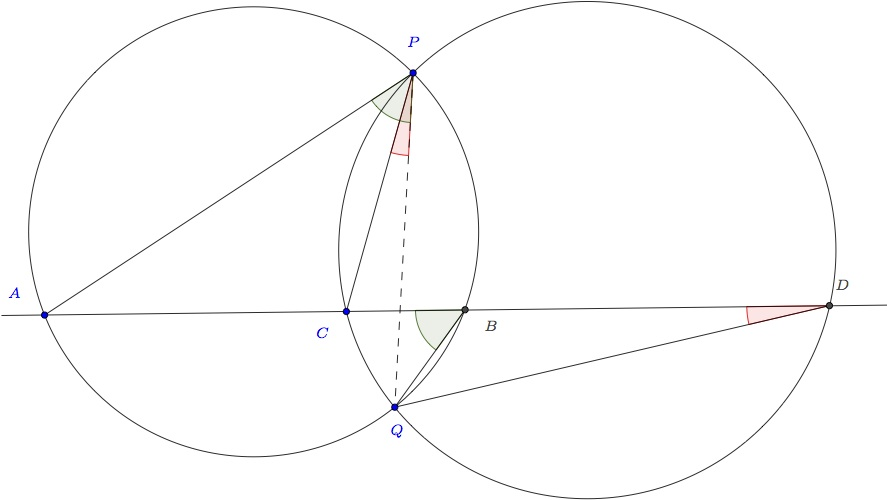
\includegraphics{../images/i11y-1}
\end{center}

Montrons que $(PA,PC)=(DQ,BQ)$. On a:
\begin{align*}
(PA,PC)&= (PA,PQ)+(PQ,PC) \\
&= (BA,BQ)+(DQ,DC) \text{ par cocyclicité dans chaque cercle}\\
&= (BA,BQ)+(DQ,BA) \text{ car $(DC)=(BA)$}\\
&= (DQ,BQ).
\end{align*}
}
}
